\documentclass[b4paper, dvipdfmx, 11pt, fleqn, twocolumn, uplatex]{jsarticle}
\usepackage{geometry}
\geometry{left=25mm,right=25mm,top=30mm,bottom=30mm}
\usepackage{graphicx}
\usepackage{amsmath}
\usepackage{amssymb}
\usepackage{ascmac}
\usepackage{setspace}
\usepackage[e]{esvect}
\usepackage{tikz}
\usetikzlibrary{arrows, calc, angles, quotes, spy, intersections, patterns, decorations.markings,decorations.pathmorphing, positioning, shapes.callouts}
\usepackage{fancybox}
\usepackage{fancyhdr}
\usepackage{dashbox}
\usepackage{wrapfig}
\usepackage{empheq}
\usepackage{siunitx}
\usepackage{tabto}
\usepackage[inline]{enumitem}
\newenvironment{tabbedenum}[1]
{\NumTabs{#1}\begin{enumerate*}[label={(\arabic*)},itemjoin={\tab}]}{\end{enumerate*}}
\renewcommand\thefootnote{\roman{footnote})}
\newcommand{\ctext}[1]{\raise0.2ex\hbox{\textcircled{\scriptsize{#1}}}}
\newcommand{\dlim}{\displaystyle \lim}
\setlength{\columnseprule}{.4pt}
\pagestyle{empty}
\pagestyle{fancy}
\parindent=0pt
\rhead{}
\cfoot{}
\let\origfrac\frac
\newcommand{\Frac}[2]{%
  \setbox0=\hbox{$#1$}\setbox1=\hbox{$#2$}\setbox2=\hbox{あ}%
  \dimen0=\wd2
  \ifdim \wd0<\dimen0
  \ifdim \wd1<\dimen0
  \origfrac{\hbox to \dimen0{\hss$#1$\hss}}{\hbox to \dimen0{\hss$#2$\hss}}%
  \else
  \origfrac{#1}{#2}%
  \fi
  \else
  \origfrac{#1}{#2}%
  \fi}

\newcommand{\sv}[1]{\vv{\mathstrut#1}}
\def\vvbar#1{\raisebox{.3ex}{$\bigl|$}\vv{#1}\raisebox{.3ex}{$\bigr|$}}
\def\svbar#1{\raisebox{.3ex}{$\bigl|$}\sv{#1}\raisebox{.3ex}{$\bigr|$}}
\newcommand{\varParallel}{\def\@varParallel{\kern .2em/\kern-.2em /\kern .2em}%
  \mathchoice%
  {\@varParallel}%
  {\textstyle\@varParallel}%
  {\scriptscriptstyle\@varParallel}%
  {\scriptscriptstyle\@varParallel}}

\newcommand{\dFrac}{\displaystyle \Frac}
\newcommand{\tria}[1]{\triangle\mathrm{#1}}


\begin{document}
\begin{screen}
次の整式の同類項をまとめて整理せよ.また,[~~]内の文字に着目したとき,その次数と定数項をいえ.
\medskip

$2a^2-ab-b^2+4ab+3a^2+2b^2$~~$[b]$
\begin{flushright}
  青チャート数1A~例題1(2)
\end{flushright}
\end{screen}
%\newpage

\begin{screen}
次の式を展開せよ.\\
\begin{tabbedenum}{2}
	\item $(x+y)(x^2+y^2)(x-y)$
	\item $(p+2q)^2(p-2q)^2$
	\item $(x+1)(x-2)(x^2-x+1)(x^2+2x+4)$
\end{tabbedenum}
\begin{flushright}
    青チャート数1A~例題8
\end{flushright}
\end{screen}

%\newpage

\begin{screen}
次の式を因数分解せよ.\\
\begin{tabbedenum}{2}
	\item $6a^3b-24ab^3$
	\item $(x^2+3x)^2-2(x^2+3x)-8$
	\item $9b^2+3ab-2a-4$
	\item $x^2-xy-2y^2-x-7y-6$
\end{tabbedenum}
\begin{flushright}
    青チャート数1A~例題10(5),12(4),14(1),15(1)
\end{flushright}
\end{screen}

%\newpage

\begin{screen}
次の値を求めよ.\\
\begin{tabbedenum}{3}
	\item $|8|$
	\item $\left|-\dFrac{2}{3}\right|$
	\item $|3-\pi|$
\end{tabbedenum}
\begin{flushright}
    青チャート数1A~例題21(1)
\end{flushright}
\end{screen}

%\newpage

\begin{screen}
$x=2, -\dFrac{1}{2}$のとき,$P=|2x+1|-|-x|$の値をそれぞれ求めよ.
\begin{flushright}
    青チャート数1A~例題21(3)
\end{flushright}
\end{screen}

%\newpage

\begin{screen}
次の(1)~(3)の場合について,$\sqrt{(a-1)^2}+\sqrt{(a-3)^2}$の根号を外し簡単にせよ.\\
\begin{tabbedenum}{3}
	\item $a\geqq3$
	\item $1\leqq a<3$
	\item $a<1$
\end{tabbedenum}
\begin{flushright}
    青チャート数1A~例題24
\end{flushright}
\end{screen}

%\newpage

\begin{screen}
連立不等式
\begin{empheq}[left=(1) \empheqlbrace]{align*}
5x+1 &\leqq 8(x+2)\\
2x-3 &<1-(x-5)
\end{empheq}
\begin{empheq}[left=(2) \empheqlbrace]{align*}
x+7 &< 1-2x\\
6x+2 &\geqq 2
\end{empheq}
を解け.
\begin{flushright}
    青チャート数1A~例題34(1), (2)
\end{flushright}
\end{screen}

%\newpage

\begin{screen}
不等式$5x-7<2x+5$を満たす自然数$x$の値をすべて求めよ.
\begin{flushright}
    青チャート数1A~例題35(1)
\end{flushright}
\end{screen}

%\newpage

\begin{screen}
次の方程式を解け.\\
\begin{tabbedenum}{2}
	\item $|x-1|=2$
	\item $|x+4|=5x$
	\item $|x-1|+|x-2|=x$
	\item $||x-4|-3|=2$
\end{tabbedenum}
\begin{flushright}
  青チャート数1A~例題39, 40
\end{flushright}
\end{screen}
%\newpage

\begin{screen}
次の不等式を解け.\\
\begin{tabbedenum}{2}
	\item $|x-2|<4$
	\item $|x+3|\geqq5$
	\item $|2x+1|\leqq3$
	\item $|x-4|<3x$
\end{tabbedenum}
\begin{flushright}
    青チャート数1A~例題41
\end{flushright}
\end{screen}

%\newpage

\begin{screen}
$U=\{1, 2, 3, 4, 5, 6, 7, 8, 9\}$を全体集合とする.\\
集合$U$の部分集合$A$, $B$を$A=\{1, 2, 4, 6, 8\}$, $B=\{1, 3, 6, 9\}$とするとき,次の集合を求めよ.\\
\begin{tabbedenum}{3}
	\item $\overline{A}$
	\item $\overline{A}\cap B$
	\item $\overline{A}\cap\overline{B}$
	\item $\overline{A}\cup\overline{B}$
	\item $\overline{A\cap B}$
	\item $\overline{A\cup B}$
\end{tabbedenum}
\begin{flushright}
    青チャート数1A~例題43
\end{flushright}
\end{screen}

%\newpage

\begin{screen}
1以上100以下の整数全体の集合$U$を全体集合として考える.\\
$A=\{x|x\mathrm{は整数の平方}, x\in U\}$,$B=\{x|x\mathrm{は偶数}, x\in U\}$,$C=\{x|x\mathrm{は4の倍数}, x\in U\}$とするとき,$\overline{C}\subset\overline{A}\cup\overline{B}$であることを示せ.
\begin{flushright}
    青チャート数1A~例題45
\end{flushright}
\end{screen}

%\newpage

\begin{screen}
$x$,$y$は実数とする.次の命題の真偽を調べよ.\\
\begin{tabbedenum}{2}
	\item $x=0$ならば$xy=0$
	\item $x^2=16$ならば$x=4$
	\item $x\ne1$ならば$x\geqq2$
	\item 「$x+y>0$かつ$xy>0$」ならば「$x>0$かつ$y>0$」
	\item $x^2+y^2=0$ならば$x=y=0$
\end{tabbedenum}
\begin{flushright}
    青チャート数1A~例題21(3)
\end{flushright}
\end{screen}

%\newpage

\begin{screen}
次の命題とその否定の真偽をそれぞれ調べよ.\\
\begin{tabbedenum}{1}
	\item すべての実数$x$について$x^2>0$
	\item ある素数は偶数である.
	\item 任意の実数$x$, $y$に対して$x^2-4xy+4y^2>0$
	\item $x^2-3x-10=0$である自然数$x$が存在する.
\end{tabbedenum}
\begin{flushright}
    青チャート数1A~例題52
\end{flushright}
\end{screen}

%\newpage

\begin{screen}
次の\fbox{\phantom{abc}}に最も適する語句を(ア)~(エ)から選べ.$x$,$y$は実数とする.\\
\begin{tabbedenum}{1}
	\item $x<1$は$x\leqq1$であるための\fbox{\phantom{abc}}.
	\item $xy+1=x+y$は$x$,$y$のうち少なくとも1つは1であるための\fbox{\phantom{abc}}.
\end{tabbedenum}\\
(ア)~~必要十分条件である\\
(イ)~~必要条件ではあるが十分条件ではない\\
(ウ)~~十分条件ではあるが必要条件ではない\\
(エ)~~必要条件でも十分条件でもない
\begin{flushright}
    青チャート数1A~例題54(1),(3)
\end{flushright}
\end{screen}

%\newpage

\begin{screen}
次の命題の逆・対偶・裏を述べ,その真偽をいえ.$x$,$a$,$b$は実数とする.
\begin{enumerate}[label={(\arabic*)}]
\item 4の倍数は2の倍数である.
\item $x=3$ならば$x^2=9$
\item $a+b>0$ならば「$a>0$かつ$b>0$」
\end{enumerate}
\begin{flushright}
    青チャート数1A~例題55
\end{flushright}
\end{screen}

%\newpage

\begin{screen}
整数$n$の平方が3ならば,$n$は3の倍数であることを証明せよ.
\begin{flushright}
    青チャート数1A~例題56
\end{flushright}
\end{screen}

%\newpage

\begin{screen}
\begin{enumerate}[label={(\arabic*)}]
\item $\sqrt{7}$は無理数であることを証明せよ.ただし,$n$を自然数とするとき,$n^2$が7の倍数ならば,$n$は7の倍数であることを用いてよいものとする.
\item $a, b$が有理数のとき,$a+b\sqrt{2}=0$ならば$a=b=0$であることを証明せよ.ただし,$\sqrt{2}$は無理数である.
\end{enumerate}
\begin{flushright}
    青チャート数1A~例題59, 60(1)
\end{flushright}
\end{screen}

%\newpage

\begin{screen}
$f(x)=4x-3$, $g(x)=-3x^2+2x$のとき,次の値を求めよ.
\begin{center}
$f\left(\dFrac{3}{2}\right), f(-2), f(a+2), g(3a), g(a-2), g(a^2)$
\end{center}
\begin{flushright}
    青チャート数1A~例題61(1)
\end{flushright}
\end{screen}

%\newpage

\begin{screen}
次の2次関数のグラフをかき,その軸と頂点を求めよ.\\
\begin{tabbedenum}{2}
	\item $y=2x^2+3x+1$
	\item $y=-x^2+4x-3$
\end{tabbedenum}
\begin{flushright}
    青チャート数1A~例題70
\end{flushright}
\end{screen}

%\newpage

\begin{screen}
放物線$y=-2x^2+4x-4$を$x$軸方向に$-3$,$y$軸方向に$1$だけ平行移動して得られる放物線の方程式を求めよ.
\begin{flushright}
    青チャート数1A~例題72
\end{flushright}
\end{screen}

%\newpage

\begin{screen}
次の関数に最大値,最小値があれば,それを求めよ.\\
\begin{tabbedenum}{2}
	\item $y=2x^2-8x+5~(0\leqq x\leqq3)$
	\item $y=-x^2-2x+2~(-3<x\leqq-2)$
\end{tabbedenum}
\begin{flushright}
    青チャート数1A~例題77
\end{flushright}
\end{screen}

%\newpage

\begin{screen}
$a$は定数とする.$0\leqq x\leqq4$における関数$f(x)=x^2-2ax+3a$について,次のものを求めよ.\\
\begin{tabbedenum}{2}
	\item 最大値
	\item 最小値
\end{tabbedenum}
\begin{flushright}
    青チャート数1A~例題79
\end{flushright}
\end{screen}

%\newpage

\begin{screen}
$a$は定数とする.$a\leqq x\leqq a+2$における関数$f(x)=x^2-2x+2$について,次のものを求めよ.\\
\begin{tabbedenum}{2}
	\item 最大値
	\item 最小値
\end{tabbedenum}
\begin{flushright}
    青チャート数1A~例題80
\end{flushright}
\end{screen}

%\newpage

\begin{screen}
\begin{tabbedenum}{2}
	\item $x+2y=3$のとき,$2x^2+y^2$の最小値を求めよ.
	\item $x\geqq0$,$y\geqq0$,$2x+y=8$のとき,$xy$の最大値と最小値を求めよ.
\end{tabbedenum}
\begin{flushright}
    青チャート数1A~例題86
\end{flushright}
\end{screen}

%\newpage

\begin{screen}
2次方程式$x^2+(a^2+a)x+a-1=0$の1つの解が$-3$であるとき,定数$a$の値を求めよ.また,そのときの他の解を求めよ.
\begin{flushright}
    青チャート数1A~例題94(2)
\end{flushright}
\end{screen}

%\newpage

\begin{screen}
$x$の2次方程式$x^2+2mx+3m+10=0$が重解をもつとき,定数$m$の値を求めよ.また,そのときの方程式の解を求めよ.
\begin{tabbedenum}{2}
	\item 最大値
	\item 最小値
\end{tabbedenum}
\begin{flushright}
    青チャート数1A~例題97(2)
\end{flushright}
\end{screen}

%\newpage

\begin{screen}
次の2次関数のグラフが$x$軸に接するように,定数$k$の値を定めよ.また,そのときの接点の座標を求めよ.
\begin{tabbedenum}{2}
	\item $y=x^2+2(2-k)x+k$
	\item $y=kx^2+3kx+3-k$
\end{tabbedenum}
\begin{flushright}
    青チャート数1A~例題102
\end{flushright}
\end{screen}

%\newpage

\begin{screen}
2次方程式$x^2+(a^2+a)x+a-1=0$の1つの解が$-3$であるとき,定数$a$の値を求めよ.また,そのときの他の解を求めよ.
\begin{flushright}
    青チャート数1A~例題94(2)
\end{flushright}
\end{screen}

%\newpage


\begin{screen}
\begin{tabbedenum}{2}
	\item $x+2y=3$のとき,$2x^2+y^2$の最小値を求めよ.
	\item $x\geqq0$,$y\geqq0$,$2x+y=8$のとき,$xy$の最大値と最小値を求めよ.
\end{tabbedenum}
\begin{flushright}
    青チャート数1A~例題86
\end{flushright}
\end{screen}

%\newpage

\begin{screen}
$\theta$は鋭角とする。
\begin{enumerate}[label={(\arabic*)}]
\item $\sin\theta=\dFrac{3}{4}$のとき,$\cos\theta$と$\tan\theta$の値を求めよ。
\item $\tan\theta=3$のとき,$\sin\theta$と$\cos\theta$の値を求めよ。
\end{enumerate}
\begin{flushright}
    青チャート数1A~例題94(2)
\end{flushright}
\end{screen}

%\newpage


\begin{screen}
\begin{enumerate}[label={(\arabic*)}]
\item 次の三角比を$\ang{45}$以下の角の三角比で表せ。\\
\begin{tabbedenum}{3}
	\item $\sin\ang{58}$
	\item $\cos\ang{56}$
	\item $\tan\ang{80}$
\end{tabbedenum}
\item $\triangle\mathrm{ABC}$の3つの内角$\angle\mathrm{A}$, $\angle\mathrm{B}$, $\angle\mathrm{C}$の大きさを,それぞれ$A$, $B$, $C$とするとき,等式$\sin\dFrac{A}{2}=\cos\dfrac{B+C}{2}$が成り立つことを証明せよ。
\end{enumerate}
\begin{flushright}
    青チャート数1A~例題135
\end{flushright}
\end{screen}

%\newpage

\begin{screen}
$\ang{0}\leqq\theta\leqq\ang{180}$のとき,次の等式を満たす$\theta$を求めよ。\\
\begin{tabbedenum}{3}
	\item $\sin\theta=\dfrac{1}{\sqrt2}$
	\item $\cos\theta=\dfrac{\sqrt3}{2}$
	\item $\tan\theta=-\dfrac{1}{\sqrt3}$
\end{tabbedenum}
\begin{flushright}
    青チャート数1A~例題138
\end{flushright}
\end{screen}

%\newpage

\begin{screen}
次の方程式を解け。
\begin{enumerate}[label={(\arabic*)}]
\item $2\cos^2\theta+3\sin\theta-3=0$~$(\ang{0}\leqq\theta\leqq\ang{180})$
\item $\sin\theta\tan\theta=-\dFrac{3}{2}$~$(\ang{90}<\theta\leqq\ang{180})$
\end{enumerate}
\begin{flushright}
    青チャート数1A~例題139
\end{flushright}
\end{screen}

%\newpage

\begin{screen}
$\ang{0}\leqq\theta\leqq\ang{180}$とする。$\cos\theta-\sin\theta=\dFrac{1}{2}$のとき,$\tan\theta$の値を求めよ。
\begin{flushright}
    青チャート数1A~例題142
\end{flushright}
\end{screen}

%\newpage

\begin{screen}
$\ang{0}\leqq\theta\leqq\ang{180}$のとき,次の不等式を満たす$\theta$の値の範囲を求めよ。\\
\begin{tabbedenum}{3}
	\item $\sin\theta>\dFrac{1}{2}$
	\item $\cos\theta\leqq\dfrac{1}{\sqrt2}$
	\item $\tan\theta<\sqrt3$
\end{tabbedenum}
\begin{flushright}
    青チャート数1A~例題144
\end{flushright}
\end{screen}

%\newpage

\begin{screen}
$\ang{0}\leqq\theta\leqq\ang{180}$のとき,次の不等式を解け。\\
\begin{tabbedenum}{3}
	\item $2\sin^2\theta-\cos\theta-1\leqq0$
	\item $2\cos^2\theta+3\sin\theta<3$
\end{tabbedenum}
\begin{flushright}
    青チャート数1A~例題145
\end{flushright}
\end{screen}

%\newpage

\begin{screen}
$\triangle{\mathrm{ABC}}$において,次のものを求めよ。
\begin{enumerate}[label={(\arabic*)}]
\item $b=\sqrt{6}$, $c=\sqrt{3}-1$, $A=\ang{45}$のとき,$a$, $B$, $C$
\item $a=1+\sqrt3$, $b=2$, $c=\sqrt6$のとき,$A$, $B$, $C$
\end{enumerate}
\begin{flushright}
    青チャート数1A~例題150
\end{flushright}
\end{screen}

%\newpage

\begin{screen}
平行四辺形ABCDで,対角線の交点を$\mathrm{O}$とすると,$\mathrm{AC}=10$, $\mathrm{BD}=6\sqrt2$, $\angle{\mathrm{AOD}}=\ang{135}$となるような四角形ABCDの面積$S$を求めよ。
\begin{flushright}
    青チャート数1A~例題159(1)
\end{flushright}
\end{screen}

%\newpage

\begin{screen}
円$\mathrm{O}$に内接する四角形ABCDは,$\mathrm{AB}=2$, $\mathrm{BC}=3$, $\mathrm{CD}=1$, $\angle{\mathrm{ABC}}=\ang{60}$を満たす。このとき,次のものを求めよ。\\
\begin{tabbedenum}{2}
	\item 線分$\mathrm{AC}$の長さ
	\item 辺$\mathrm{AD}$の長さ
	\item 円$\mathrm{O}$の半径
	\item 四角形ABCDの面積
\end{tabbedenum}
\begin{flushright}
    青チャート数1A~例題162
\end{flushright}
\end{screen}

%\newpage


%ここから『データの分析』

\begin{screen}
次のデータは,ある商品A, Bの5日間の売上個数である。\\
A: $5, 7, 4, 3, 6$\quad B: $4, 6, 8, 3, 9$\quad(単位は個)\\
A, Bの変量をそれぞれ$x$, $y$とするとき,次の問いに答えよ。
\begin{enumerate}[label={(\arabic*)}]
\item $x$, $y$のデータの平均値,分散,標準偏差をそれぞれ求めよ。ただし標準偏差については小数第2位を四捨五入せよ。
\item $x$, $y$のデータについて,標準偏差によってデータの平均値からの散らばり度合いを比較せよ。
\end{enumerate}
\begin{flushright}
    青チャート数1A~例題177
\end{flushright}
\end{screen}

%\newpage

\begin{screen}
変量$x$のデータの平均値$\overline{x}$が$\overline{x}=21$,分散${s_x}^2$が${s_x}^2=12$であるとする。このとき,次の式によって得られる新しい変量$y$のデータについて,平均値$\overline{y}$,分散${s_y}^2$,標準偏差$s_y$を求めよ。\\
ただし,$\sqrt3=1.73$とし,標準偏差は小数第2位を四捨五入して,小数第1位まで求めよ。\\
\begin{tabbedenum}{2}
\item $y=x-5$
\item $y=3x$
\item $y=-2x+3$
\item $y=\dfrac{x-21}{2\sqrt3}$
\end{tabbedenum}
\begin{flushright}
    青チャート数1A~例題180
\end{flushright}
\end{screen}

%\newpage

\begin{screen}
次の表は,学生5名の身長$x$~(\si{cm})と体重$y$~(\si{kg})を測定した結果である。$x$と$y$の相関係数$r$を求めよ。
\begin{center}
  \begin{tabular}{c||c|c|c|c|c} \hline
    &  A& B & C & D & E \\ \hline
    身長$x$~(\si{cm}) &181 & 167 & 173 & 169 & 165 \\
    体重$y$~(\si{kg}) & 75 & 59 & 63 & 67 & 61\\
    \hline
  \end{tabular}
\end{center}
\begin{flushright}
    青チャート数1A~例題183
\end{flushright}
\end{screen}

%\newpage

%ここから数A『場合の数』

\begin{screen}
\begin{enumerate}[label={(\arabic*)}]
\item 大小2個のさいころを投げるとき,出る目の和が5の倍数になる場合は何通りにあるか。
\item $(a+b+c)(p+q+r)(x+y)$を展開すると,異なる項は何個できるか。
\end{enumerate}
\begin{flushright}
    青チャート数1A~例題7
\end{flushright}
\end{screen}

%\newpage

\begin{screen}
540の正の約数は全部で何個あるか。また,その約数の和を求めよ。
\begin{flushright}
    青チャート数1A~例題8
\end{flushright}
\end{screen}

%\newpage

\begin{screen}
$0,1, 2, ,3 ,4 5$の6個の数字から異なる4個の数字を取って並べて,4桁の整数を作るものとする。次のものは全部で何個できるか。\\
\begin{tabbedenum}{2}
	\item 整数
	\item 3の倍数
	\item 6の倍数
	\item 2400より大きい整数
\end{tabbedenum}
\begin{flushright}
    青チャート数1A~例題12
\end{flushright}
\end{screen}

%\newpage

\begin{screen}
男子A, B, C, 女子D, E, F, Gの7人が1列に並ぶとき
\begin{enumerate}[label={(\arabic*)}]
\item AとBが隣り合うような並べ方は全部で何通りあるか。
\item AとBが両端にくるような並び方は全部で何通りあるか。
\item どの男子も隣り合わないような並び方は全部で何通りあるか。
\end{enumerate}
\begin{flushright}
    青チャート数1A~例題13
\end{flushright}
\end{screen}

%\newpage

\begin{screen}
9人を次のように分ける方法は何通りあるか。
\begin{enumerate}[label={(\arabic*)}]
\item 4人,3人,2人の3組に分ける。
\item 3人ずつ,A, B, Cの3組に分ける。
\item 3人ずつ3組に分ける。
\item 5人,2人,2人の3組に分ける。
\end{enumerate}
\begin{flushright}
    青チャート数1A~例題26
\end{flushright}
\end{screen}

%\newpage

\begin{screen}
YOKOHAMAの8文字を横1列に並べて順列を作るとき,次の数を求めよ。
\begin{enumerate}[label={(\arabic*)}]
\item 順列の総数
\item AAとOOという並びをともに含む順列の数
\item Y, K, H, Mがこの順に並ぶ順列の数
\end{enumerate}
\begin{flushright}
    青チャート数1A~例題29
\end{flushright}
\end{screen}

%\newpage

\begin{screen}
袋Aには赤玉3個と青玉2個,袋Bには赤玉7個と青玉3個が入っている。
\begin{enumerate}[label={(\arabic*)}]
\item 袋Aから1個,袋Bから2個の玉を取り出すとき,玉の色がすべて同じである確率を求めよ。
\item 袋Aには白玉1個を加える。袋Aから玉を1個取り出し,色を確認した後,もとに戻す。これを3回繰り返すとき,すべての色の玉が出る確率を求めよ。
\end{enumerate}
\begin{flushright}
    青チャート数1A~例題48
\end{flushright}
\end{screen}

%\newpage

\begin{screen}
あるゲームでAがBに勝つ確率は常に一定で$\dFrac{3}{5}$とする。A, Bがゲームをし,先に3ゲーム勝った方を優勝とする大会を行う。このとき,3ゲーム目で優勝が決まる確率は${}^{\mathrm{ア}}\fbox{\phantom{AA}}$である。また,5ゲーム目まで行って,Aが優勝する確率は${}^{\mathrm{イ}}\fbox{\phantom{AA}}$である。ただし,ゲームでは必ず勝負がつくものとする。
\begin{flushright}
    青チャート数1A~例題50
\end{flushright}
\end{screen}

%\newpage

\begin{screen}
10本のくじの中に当たりくじが3本ある。一度引いたくじはもとに戻さない。
\begin{enumerate}[label={(\arabic*)}]
\item 初めにaは1本引き,次にbが1本引くとき,次の確率を求めよ。\\
\begin{tabbedenum}{2}
	\item a, bともに当たる確率
	\item bが当たる確率
\end{tabbedenum}
\item 初めaが1本ずつ2回引き,次にbが1本引くとき,a, bが1本ずつ当たる確率を求めよ。
\end{enumerate}
\begin{flushright}
    青チャート数1A~例題59
\end{flushright}
\end{screen}

%\newpage

\begin{screen}
ある工場では,同じ製品をいくつかの機械で製造している。不良品が現れる確率は機械Aの場合は\SI{4}{\%}であるが,それ以外の機械では\SI{7}{\%}に上がる。また,機械Aで製品全体の\SI{60}{\%}を作る。製品の中から1個を取り出したとき
\begin{enumerate}[label={(\arabic*)}]
\item それが不良品である確率を求めよ。
\item 不良品であったとき,それが機械Aの製品である確率を求めよ。
\end{enumerate}
\begin{flushright}
    青チャート数1A~例題62
\end{flushright}
\end{screen}

%\newpage

%ここから『図形の性質』

\begin{screen}
$\triangle{\mathrm{ABC}}$において,辺BCの中点をMとし,$\angle{\mathrm{AMB}}$,$\angle{\mathrm{AMC}}$の二等分線が辺AB, ACと交わる点をそれぞれD, Eとする。このとき,$\mathrm{DE}\varParallel\mathrm{BC}$であることを証明せよ。
\begin{enumerate}[label={(\arabic*)}]
\item 4人,3人,2人の3組に分ける。
\item 3人ずつ,A, B, Cの3組に分ける。
\item 3人ずつ3組に分ける。
\item 5人,2人,2人の3組に分ける。
\end{enumerate}
\begin{flushright}
    青チャート数1A~例題65
\end{flushright}
\end{screen}

%\newpage

\begin{screen}
\begin{enumerate}[label={(\arabic*)}]
\item $\triangle{ABC}$の内心をI,点DをAIとBCの交点とする。$\alpha=\angle\mathrm{CID}$, $\beta=\angle\mathrm{BDI}$,$\angle\mathrm{BAI}=\ang{35}$, $\angle\mathrm{ACI}=\ang{30}$とする。このとき,角$\alpha$, $\beta$を求めよ。
\item $\triangle{\mathrm{ABC}}$の内心をIとし,直線AIと辺BCの交点をDとする。$\mathrm{AB}=8$, $\mathrm{BC}=7$, $\mathrm{AC}=4$であるとき,$\mathrm{AI}:\mathrm{ID}$を求めよ。
\end{enumerate}
\begin{flushright}
    青チャート数1A~例題68
\end{flushright}
\end{screen}

%\newpage

\begin{screen}
\begin{enumerate}[label={(\arabic*)}]
\item 1辺の長さが7の正三角形ABCがある。辺AB, AC上に$\mathrm{AD}=3$, $\mathrm{AE}=6$となるように2点D, Eをとる。このとき,BE, CDの交点F, 直線AFとBCとの交点をGとする。線分CGの長さを求めよ。
\item $\triangle{\mathrm{ABC}}$において,辺AB上と辺ACの延長上にそれぞれ点E, Fをとり,$\mathrm{AE}:\mathrm{EB}=1:2$, $\mathrm{AF}:\mathrm{FC}=3:1$とする。直線EFと直線BCとの交点をDとするとき,$\mathrm{BD}:\mathrm{DC}$, $\mathrm{ED}:\mathrm{DF}$をそれぞれ求めよ。
\end{enumerate}
\begin{flushright}
    青チャート数1A~例題76
\end{flushright}
\end{screen}

%\newpage

\begin{screen}
下の図で,四角形ABCDは円に内接している。角$\theta$を求めよ。\\
\begin{tabbedenum}{2}
\item %
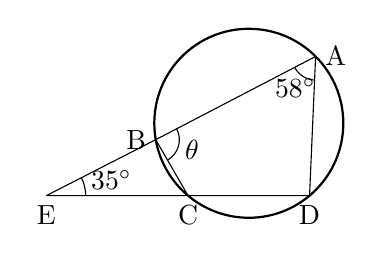
\begin{tikzpicture}[rotate=0, scale=0.6, baseline={( [yshift=-11pt] current bounding box.north)}]
\coordinate (O) at (0,0);
\coordinate (A) at (45:2) node at (A) [right] {A};
\coordinate (B) at (190:2) node at (B) [left] {B};
\coordinate (C) at (230:2) node at (C) [below] {C};
\coordinate (D) at (310:2) node at (D) [below] {D};
\coordinate (E) at ($ (C)!3cm!130:(O) $) node at (E) [below] {E};
\draw[name path=circleO, thick] (O) circle (2);
\draw(E)--($ (E)!1.85!(C) $);
\draw [name path=E--B--(A)](E)--(B)--(A);
\draw(A)--(D);
\draw(B)--(C);
\pic [draw,"$\theta$",angle radius=0.3cm,angle eccentricity=1.6] {angle=C--B--A};
\pic [draw,"$\ang{35}$",angle radius=0.5cm,angle eccentricity=1.7] {angle=C--E--B};
\pic [draw,"$\ang{58}$",angle radius=0.3cm,angle eccentricity=1.6] {angle=B--A--D};
\end{tikzpicture}
\item %
\begin{tikzpicture}[rotate=0, scale=0.6, baseline={( [yshift=-11pt] current bounding box.north)}]
\coordinate (O) at (0,0);
\coordinate (A) at (230:2) node at (C) [below] {A};
\coordinate (B) at (310:2) node at (D) [below] {B};
\coordinate (E) at ($ (B)!1.6cm!-130:(O) $) node at (E) [below] {E};
\coordinate (C) at (7:2) node at (C) [right] {C};
\coordinate (D) at (45:2) node at (D) [left] {D};
\coordinate (F) at ($ (C)!3cm!243:(O) $) node at (F) [right] {F};
\draw[name path=circleO, thick] (O) circle (2);
\draw(E)--($ (E)!1.7!(C) $);
\draw [name path=E--B--(A)](E)--(B)--(A);
\draw(C)--(F);
\draw(F)--(D);
\draw(A)--(D);
\draw(B)--(C);
\pic [draw,"$\theta$",angle radius=0.3cm,angle eccentricity=1.6] {angle=B--A--D};
\pic [draw,"$\ang{60}$",angle radius=0.3cm,angle eccentricity=1.6] {angle=C--E--B};
\pic [draw,"$\ang{20}$",angle radius=0.6cm,angle eccentricity=1.6] {angle=D--F--C};
\end{tikzpicture}
\end{tabbedenum}
\begin{flushright}
    青チャート数1A~例題59
\end{flushright}
\end{screen}

%\newpage

\begin{screen}
ある工場では,同じ製品をいくつかの機械で製造している。不良品が現れる確率は機械Aの場合は\SI{4}{\%}であるが,それ以外の機械では\SI{7}{\%}に上がる。また,機械Aで製品全体の\SI{60}{\%}を作る。製品の中から1個を取り出したとき
\begin{enumerate}[label={(\arabic*)}]
\item それが不良品である確率を求めよ。
\item 不良品であったとき,それが機械Aの製品である確率を求めよ。
\end{enumerate}
\begin{flushright}
    青チャート数1A~例題62
\end{flushright}
\end{screen}

%\newpage


\begin{screen}
$\triangle{\mathrm{ABC}}$において,辺BCの中点をMとし,$\angle{\mathrm{AMB}}$,$\angle{\mathrm{AMC}}$の二等分線が辺AB, ACと交わる点をそれぞれD, Eとする。このとき,$\mathrm{DE}\varParallel\mathrm{BC}$であることを証明せよ。
\begin{enumerate}[label={(\arabic*)}]
\item 4人,3人,2人の3組に分ける。
\item 3人ずつ,A, B, Cの3組に分ける。
\item 3人ずつ3組に分ける。
\item 5人,2人,2人の3組に分ける。
\end{enumerate}
\begin{flushright}
    青チャート数1A~例題65
\end{flushright}
\end{screen}

%\newpage

\begin{screen}
\begin{enumerate}[label={(\arabic*)}]
\item $\triangle{ABC}$の内心をI,点DをAIとBCの交点とする。$\alpha=\angle\mathrm{CID}$, $\beta=\angle\mathrm{BDI}$,$\angle\mathrm{BAI}=\ang{35}$, $\angle\mathrm{ACI}=\ang{30}$とする。このとき,角$\alpha$, $\beta$を求めよ。
\item $\triangle{\mathrm{ABC}}$の内心をIとし,直線AIと辺BCの交点をDとする。$\mathrm{AB}=8$, $\mathrm{BC}=7$, $\mathrm{AC}=4$であるとき,$\mathrm{AI}:\mathrm{ID}$を求めよ。
\end{enumerate}
\begin{flushright}
    青チャート数1A~例題68
\end{flushright}
\end{screen}

%\newpage

%ここから『式と証明』

\begin{screen}
$(a-2b)^6$の展開式で,$a^5b$の項の係数は${}^{ア}\fbox{\phantom{AA}}$,$a^2b^4$の項の係数は${}^{イ}\fbox{\phantom{AA}}$である。また,$\left(x^2-\dFrac{2}{x}\right)^6$の展開式で,$x^6$の項の係数は${}^{ウ}\fbox{\phantom{AA}}$,定数項は${}^{エ}\fbox{\phantom{AA}}$である。
\begin{flushright}
    青チャート数2B~例題2
\end{flushright}
\end{screen}

%\newpage

\begin{screen}
次の等式が$x$についての恒等式となるように,定数$a$, $b$, $c$の値を定めよ。
\[
\dfrac{-2x^2+6}{(x+1)(x-1)^2}=\dfrac{a}{x+1}-\dfrac{b}{x-1}+\dfrac{c}{(x-1)^2}
\]
\begin{flushright}
    青チャート数2B~例題17
\end{flushright}
\end{screen}

%\newpage

\begin{screen}
  \begin{enumerate}[label={(\arabic*)}]
    \item $\dfrac{x+y}{5}=\dfrac{y+z}{6}=\dfrac{z+x}{7}(\neq0)$のとき,$\dfrac{xy+yz+zx}{x^2+y^2+z^2}$の値を求めよ。
    \item $\dfrac{b+c}{a}=\dfrac{c+a}{b}=\dfrac{a+b}{c}$のとき,この式の値を求めよ。
  \end{enumerate}
\begin{flushright}
    青チャート数2B~例題24
\end{flushright}
\end{screen}

%\newpage

\begin{screen}
  次の不等式を証明せよ。また,等号が成り立つのはどのゆなときか。
  \begin{enumerate}[label={(\arabic*)}]
    \item $x^2-6xy+10y^2\geqq4y-4$
    \item $(a^2+b^2)(x^2+y^2)\geqq(ax+by)^2$
  \end{enumerate}
  \begin{flushright}
      青チャート数2B~例題27
  \end{flushright}
\end{screen}

%\newpage

\begin{screen}
$a$, $b$は正の数とする。次の不等式が成り立つことを証明せよ。また,等号が成り立つのはどのようなときか。
  \begin{enumerate}[label={(\arabic*)}]
    \item $a+\dFrac{4}{a}\geqq4$
    \item $\left(a+\dFrac{1}{b}\right)\left(b+\dFrac{4}{a}\right)\geqq9$
  \end{enumerate}
\begin{flushright}
    青チャート数2B~例題31
\end{flushright}
\end{screen}

%\newpage

\begin{screen}
  \begin{enumerate}[label={(\arabic*)}]
    \item $x>0$のとき,$x+\dfrac{16}{x+2}$の最小値を求めよ。
    \item $x>0$, $y>0$とする。$(3x+2y)\left(\dFrac{3}{x}+\dFrac{2}{y}\right)$の最小値を求めよ。
  \end{enumerate}
\begin{flushright}
    青チャート数2B~例題32
\end{flushright}
\end{screen}

%\newpage

%ここから『複素数と方程式』

\begin{screen}
次の等式を満たす実数$x$, $y$の値を,それぞれ求めよ。
  \begin{enumerate}[label={(\arabic*)}]
    \item $(4+2i)x+(1+4i)y+7=0$
    \item $(x+2yi)(1+i)=3-2i$
  \end{enumerate}
\begin{flushright}
    青チャート数2B~例題100
\end{flushright}
\end{screen}

%\newpage

\begin{screen}
2円$x^2+y^2=r^2~(r>0)\cdots\ctext{1}$,$x^2+y^2-8x-4y+4=0\cdots\ctext{2}$について
\begin{enumerate}[label={(\arabic*)}]
\item 円\ctext{1}と円\ctext{2}が内接するとき,定数$r$の値を求めよ。
\item 円\ctext{1}と円\ctext{2}が異なる2点で交わるとき,定数$r$の値の範囲を求めよ。
\end{enumerate}
\begin{flushright}
    青チャート数2B~例題103
\end{flushright}
\end{screen}

%\newpage

%ここから『図形と方程式』

\begin{screen}
3点A$(5, 4)$, B$(0, -1)$, C$(8, -2)$について,線分ABを$2:3$に外分する点をP, $3:2$に外分する点をQとし,$\tria{ABC}$の重心をGとする。
\begin{enumerate}[label={(\arabic*)}]
\item 線分PQの中点Mの座標を求めよ。
\item 点Gの座標を求めよ。
\item $\tria{PQS}$の重心が点Gと一致するように,点Sの座標を定めよ。
\end{enumerate}
\begin{flushright}
    青チャート数2B~例題73
\end{flushright}
\end{screen}

%\newpage

\begin{screen}
点$(-3,2)$を通り,直線$3x-4y-6=0$に平行な直線$l$と垂直な直線$l'$の方程式をそれぞれ求めよ。
\begin{flushright}
    青チャート数2B~例題77
\end{flushright}
\end{screen}

%\newpage

\begin{screen}
$xy$平面上に2点A$(3, 2)$,B$(8, 9)$がある。点Pが直線$l:y=x-3$上を動くとき,$\mathrm{AP}+\mathrm{PB}$の最小値と,そのときの点Pの座標を求めよ。
\begin{flushright}
    青チャート数2B~例題87
\end{flushright}
\end{screen}

%\newpage

\begin{screen}
\begin{enumerate}[label={(\arabic*)}]
\item 点(2, 8)と直線$3x-2y+4=0$の距離を求めよ。
\item 平行な2直線$5x+4y=20$,$5x+4y=60$間の距離を求めよ。
\item 点$(2,1)$から直線$kx+y+1=0$に下ろした垂線の長さが$\sqrt{3}$であるとき,定数$k$の値を求めよ。
\end{enumerate}
\begin{flushright}
    青チャート数2B~例題88
\end{flushright}
\end{screen}

%\newpage

\begin{screen}
次の円の方程式を求めよ。
\begin{enumerate}[label={(\arabic*)}]
\item $x$軸と$y$軸の両方に接し,点A$(-4, 2)$を通る。
\item 点A$(1, 1)$を通り,$y$軸に接し,中心が直線$y=2x$上にある。
\end{enumerate}
\begin{flushright}
    青チャート数2B~例題94
\end{flushright}
\end{screen}

%\newpage

\begin{screen}
直線$y=x+2$が円$x^2+y^2=5$によって切り取られる弦の長さを求めよ。
\begin{flushright}
    青チャート数2B~例題97
\end{flushright}
\end{screen}

%\newpage

\begin{screen}
点P$(-5, 10)$を通り,円$x^2+y^2=25$に接する直線の方程式を求めよ。
\begin{flushright}
    青チャート数2B~例題100
\end{flushright}
\end{screen}

%\newpage

\begin{screen}
2円$x^2+y^2=r^2~(r>0)\cdots\ctext{1}$,$x^2+y^2-8x-4y+4=0\cdots\ctext{2}$について
\begin{enumerate}[label={(\arabic*)}]
\item 円\ctext{1}と円\ctext{2}が内接するとき,定数$r$の値を求めよ。
\item 円\ctext{1}と円\ctext{2}が異なる2点で交わるとき,定数$r$の値の範囲を求めよ。
\end{enumerate}
\begin{flushright}
    青チャート数2B~例題103
\end{flushright}
\end{screen}

%\newpage

\begin{screen}
2点A$(-4, 0)$,B$(2, 0)$からの距離の比が$2:1$である点の軌跡を求めよ。
\begin{flushright}
    青チャート数2B~例題107
\end{flushright}
\end{screen}

%\newpage

%ここから『図形と方程式』

\begin{screen}
3点A$(5, 4)$, B$(0, -1)$, C$(8, -2)$について,線分ABを$2:3$に外分する点をP, $3:2$に外分する点をQとし,$\tria{ABC}$の重心をGとする。
\begin{enumerate}[label={(\arabic*)}]
\item 線分PQの中点Mの座標を求めよ。
\item 点Gの座標を求めよ。
\item $\tria{PQS}$の重心が点Gと一致するように,点Sの座標を定めよ。
\end{enumerate}
\begin{flushright}
    青チャート数2B~例題73
\end{flushright}
\end{screen}

%\newpage

\begin{screen}
点$(-3,2)$を通り,直線$3x-4y-6=0$に平行な直線$l$と垂直な直線$l'$の方程式をそれぞれ求めよ。
\begin{flushright}
    青チャート数2B~例題77
\end{flushright}
\end{screen}

%\newpage

\begin{screen}
$xy$平面上に2点A$(3, 2)$,B$(8, 9)$がある。点Pが直線$l:y=x-3$上を動くとき,$\mathrm{AP}+\mathrm{PB}$の最小値と,そのときの点Pの座標を求めよ。
\begin{flushright}
    青チャート数2B~例題87
\end{flushright}
\end{screen}

%\newpage

\begin{screen}
\begin{enumerate}[label={(\arabic*)}]
\item 点(2, 8)と直線$3x-2y+4=0$の距離を求めよ。
\item 平行な2直線$5x+4y=20$,$5x+4y=60$間の距離を求めよ。
\item 点$(2,1)$から直線$kx+y+1=0$に下ろした垂線の長さが$\sqrt{3}$であるとき,定数$k$の値を求めよ。
\end{enumerate}
\begin{flushright}
    青チャート数2B~例題88
\end{flushright}
\end{screen}

%\newpage

\begin{screen}
次の円の方程式を求めよ。
\begin{enumerate}[label={(\arabic*)}]
\item $x$軸と$y$軸の両方に接し,点A$(-4, 2)$を通る。
\item 点A$(1, 1)$を通り,$y$軸に接し,中心が直線$y=2x$上にある。
\end{enumerate}
\begin{flushright}
    青チャート数2B~例題94
\end{flushright}
\end{screen}

%\newpage

\begin{screen}
直線$y=x+2$が円$x^2+y^2=5$によって切り取られる弦の長さを求めよ。
\begin{flushright}
    青チャート数2B~例題97
\end{flushright}
\end{screen}

%\newpage

\begin{screen}
点P$(-5, 10)$を通り,円$x^2+y^2=25$に接する直線の方程式を求めよ。
\begin{flushright}
    青チャート数2B~例題100
\end{flushright}
\end{screen}

%\newpage

\begin{screen}
2円$x^2+y^2=r^2~(r>0)\cdots\ctext{1}$,$x^2+y^2-8x-4y+4=0\cdots\ctext{2}$について
\begin{enumerate}[label={(\arabic*)}]
\item 円\ctext{1}と円\ctext{2}が内接するとき,定数$r$の値を求めよ。
\item 円\ctext{1}と円\ctext{2}が異なる2点で交わるとき,定数$r$の値の範囲を求めよ。
\end{enumerate}
\begin{flushright}
    青チャート数2B~例題103
\end{flushright}
\end{screen}

%\newpage

\begin{screen}
2点A$(-4, 0)$,B$(2, 0)$からの距離の比が$2:1$である点の軌跡を求めよ。
\begin{flushright}
    青チャート数2B~例題107
\end{flushright}
\end{screen}

%\newpage

\begin{screen}
放物線$y=x^2+(2t-10)x-4t+16$の頂点をPとする。$t$が0以上の値をとって変化するとき,頂点Pの軌跡を求めよ。
\begin{flushright}
    青チャート数2B~例題110
\end{flushright}
\end{screen}


%ここから『平面ベクトル』

\begin{screen}
\begin{enumerate}[label={(\arabic*)}]
\item 次の等式が成り立つことを証明せよ。
\[ \vv{\textrm{AB}}+\vv{\textrm{EC}}+\vv{\textrm{FD}}=\vv{\textrm{EB}}+\vv{\textrm{FC}}+\vv{\textrm{AD}} \]
\item %
\begin{enumerate}[label={(i)}]
\item $\sv{x}=2\sv{a}-3\sv{b}-c$, $\sv{y}=-4\sv{a}+5\sv{b}-3\sv{c}$のとき,$\sv{x}-\sv{y}$を$\sv{a}, \sv{b}, \sv{c}$で表せ。
\item $4\sv{x}-3\sv{a}=\sv{x}+6\sv{b}$を満たす$\sv{x}$を$\sv{a}, \sv{b}$で表せ。
\item $3\sv{x}+\sv{y}=\sv{a}$, $5\sv{x}+2\sv{y}=\sv{b}$を満たす$\sv{x}$, $\sv{y}$を$\sv{a}$, $\sv{b}$で表せ。
\end{enumerate}
\end{enumerate}
\begin{flushright}
    青チャート数2B~例題2
\end{flushright}
\end{screen}

%\newpage

\begin{screen}
正六角形ABCDEFにおいて,中心O,辺CDを$2:1$に内分する点をP, 辺EFの中点をQとする。$\sv{\textrm{AB}}=\sv{a}$, $\sv{\textrm{AF}}=\sv{b}$とするとき,ベクトル$\sv{\textrm{BC}}$, $\sv{\textrm{EF}}$, $\sv{\textrm{CE}}$, $\sv{\textrm{AC}}$, $\sv{\textrm{BD}}$, $\sv{\textrm{QP}}$をそれぞれ$\sv{a}$, $\sv{b}$で表せ。
\begin{flushright}
    青チャート数2B~例題4
\end{flushright}
\end{screen}

%\newpage

\begin{screen}
$t$は実数とする。$\sv{a}=(2, 1)$, $\sv{b}=(3, 4)$に対して,$\left|\sv{a}+t\sv{b}\right|$は$t={}^{\textrm{ア}}\fbox{\phantom{AB}}$のとき最小値${}^{\textrm{イ}}\fbox{\phantom{AB}}$をとる。
\begin{flushright}
    青チャート数2B~例題9
\end{flushright}
\end{screen}

%\newpage

\begin{screen}
\begin{enumerate}[label={(\arabic*)}]
\item $p$を正の数とし,ベクトル$\sv{a}=(1, 1)$と$\sv{b}=(1, -p)$があるとする。いま,$\sv{a}$と$\sv{b}$のなす角が$\ang{60}$のとき,$p$の値を求めよ。
\item $\sv{a}=(-1, 3)$と$\sv{b}=(m, n)$~($m$と$n$は正の数), $\vvbar{b}=\sqrt{5}$のとき,$\sv{a}$, $\sv{b}$のなす角は$\ang{45}$である。このとき,$m$, $n$の値を求めよ。
\end{enumerate}
\begin{flushright}
    青チャート数2B~例題12
\end{flushright}
\end{screen}

\end{document}
